\chapter{L'entropie}
Il est intéressant de donner une formulation quantitative au second principe ; 
c'est l'objectif de ce chapitre.

	\section{L'inégalité de Clausius}
	Cette inégalité est un corollaire du second principe :\\
	
	\proposition{Pour tout système fermé à température uniforme décrivant un cycle,
	\begin{equation}
	\oint \dfrac{\delta Q}{T} \leq 0
	\end{equation}
	où $\delta Q$ est la quantité de chaleur reçue sur un élément de cycle, et $T$ 
	la température du système à l'état correspondant.}\ 
	
	\begin{proof}\ \\
	Vérifions cette inégalité sur le cycle de Carnot. Ce cycle réversible : les 
	échanges sont isothermes :
	\begin{equation}
	\oint \dfrac{\delta Q}{T} = \dfrac{Q_C}{T_C} - \dfrac{Q_F^*}{T_F} = 0
	\end{equation}
	L'intégalité est bien vérifiée, toute la source "chaude" va intégralement vers 
	la "froide". Vérifions maintenant que ça soit toujours le 
	cas pour un cycle irréversible\footnote{On considère des parties réversibles, 
	d'autre pas.} : le cycle étant irréversible $W_{irr}^* < W_{rev}^*$ et donc 
	$Q_{F,irr}^* > Q_{F,rev}^*$. On a donc 
	\begin{equation}
	\int_C \dfrac{\delta Q}{T} = \int_C \dfrac{\delta Q}{T_C} = \dfrac{Q_C}{T_C}, 
	\qquad\qquad
	\int_F \dfrac{\delta Q^*}{T} = \int_F \dfrac{\delta Q^*}{T_F} = \dfrac{Q_{F,irr}^*}{T_F} 
	> \dfrac{Q_{F,rev}^*}{T_F} 
	\end{equation}
	On peut directement sortir $Q_C$ de l'intégrale. La dernière inégalité (stricte) 
	provient de l'irréversibilité, provoquant une dégradation de l'énergie. En 
	soustrayant\footnote{L'idée est de faire "apparaître" la relation pour le cycle 
	de Carnot réversible qui est bien nulle en "minorant" l'intégrale.}
	\begin{equation}
	\oint \dfrac{\delta Q}{T} = \int_C \dfrac{\delta Q}{T}-\int_F\dfrac{\delta Q}{T} 
	< \dfrac{Q_C}{T_C}-\dfrac{Q_{F,rev}^*}{T_F} = 0
	\end{equation}
	Un cycle de Carnot frigorifique n'est qu'un cycle de Carnot inversé qui lui 
	aussi satisfait\footnote{On vérifié pour pour un cycle frigorifique, c'est 
	aussi valable pour clore la démonstration.}
	\begin{equation}
	\oint \dfrac{\delta Q}{T} = \dfrac{Q_F}{T_F}-\dfrac{Q_C^*}{T_C} = 0
	\end{equation}
	Ce cycle passe par le même chemin en prélevant la même quantité de chaleur à la 
	source froide $Q_F$ mais avec certaines parties du parcours irréversibles : 
	$W_{irr} > W_{rev} ; Q_{C,irr}^* > Q_{C,rev}^*$. Il en résulte
	\begin{equation}
	\int_F \dfrac{\delta Q}{T} = \int_F \dfrac{\delta Q}{T_F} = \dfrac{Q_F}{T_F}, 
	\qquad\qquad
	\int_C \dfrac{\delta Q^*}{T} = \int_F \dfrac{\delta Q^*}{T_C} = \dfrac{Q_{C,irr}^*}{T_C} 
	> \dfrac{Q_{C,rev}^*}{T_C} 
	\end{equation}
	En 	soustrayant
	\begin{equation}
	\oint \dfrac{\delta Q}{T} = \int_F \dfrac{\delta Q}{T}-\int_C\dfrac{\delta Q}{T} 
	< \dfrac{Q_F}{T_F}-\dfrac{Q_{C,rev}^*}{T_C} = 0
	\end{equation}
	Ce qui complète la démonstration de la proposition.
	\end{proof}
	
	
	\section{L'entropie}
	Soit deux cycles réversibles : $A,B$ ; $A,C$. Comme ils sont réversibles  :
	\begin{equation}
	\oint \dfrac{\delta Q}{T} = \int_1^2 \left(\dfrac{\delta Q}{T}\right)_A + 
	\int_2^1 \left(\dfrac{\delta Q}{T}\right)_B = 0
	\end{equation}
	et
	\begin{equation}
		\oint \dfrac{\delta Q}{T} = \int_1^2 \left(\dfrac{\delta Q}{T}\right)_A + 
	\int_2^1 \left(\dfrac{\delta Q}{T}\right)_C = 0
	\end{equation}
	Après soustraction
	\begin{equation}
	\int_2^1 \left(\dfrac{\delta Q}{T}\right)_B = \int_2^1 \left(\dfrac{\delta 
	Q}{T}\right)_C
	\end{equation}
	Forcément, cette entropie doit être la même : l'intégrale ne dépend pas du 
	chemin parcouru et ça sent bon pour formé une variable d'état (différentielle 
	exacte).\\
	La relation suivante est importante, car elle indique que la différence entre 
	deux états n'est pas fonction du parcours (réversible ou non) \textbf{mais} 
	pour calculer cette différence il faut imaginer un parcours réversible et 
	calculer :
	\begin{equation}
	dS = \left(\dfrac{\delta Q}{T}\right)_{rev}
	\end{equation}
	il s'agit de l'\textbf{entropie}. Si le parcours n'est pas réversible, on ne 
	sait pas comment $T$ varie et on ne peut pas calculer !
	
	\section{L’entropie d’une substance pure}
	On peut rentre l'entropie, extensive, en une variable intensive : l'entropie 
	massique $s$. On la lie au titre par la relation
	\begin{equation}
	s = (1-x)s_l + xs_g = s_l + x(s_g-s_l)
	\end{equation}
	
	
	\section{Les variations d’entropie au cours de transformations réversibles}
		\subsection{Le cycle de Carnot}
		Le cycle de Carnot se décompose en quatre transformations
		\begin{enumerate}
		\item \textit{Chauffage isotherme}.\\
		On a 
		\begin{equation}
		S_2-S_1 = \int_1^2 \dfrac{\delta Q}{T} = \dfrac{_1Q_2}{T_C}
		\end{equation}
		avec $_1Q_2$ l'aire $1-2-b-a-1$.
		\item \textit{Détente adiabatique}.\\
		Adiabatique et réversible, $dS=0$. Le segment vertical $2-3$ est dit 
		isentropique.
		\item \textit{Refroidissement isotherme}.\\
		Comme pour 1-2, on a
		\begin{equation}
		S_4-S_3 = \int_3^4 \dfrac{\delta Q}{T} = \dfrac{_3Q_4}{T_4}
		\end{equation}		
		grandeur négative car $_3Q_4<0$. La chaleur cédée à la source froide est 
		l'aire $3-4-a-b-3$.
		\item \textit{Compression adiabatique}.\\
		Même topo, $dS=0$.
		\end{enumerate}
		Le travail net du cycle $W^*$ valant la chaleur nette reçue, il correspond 
		à l'aire $1-2-3-4$ et exprimer le rendement 
		\begin{equation}
		\epsilon_{th} = \dfrac{W^*}{Q_C} = \frac{\text{aire} 1-2-3-4-1}{\text{aire} 
		1-2-b-a-1}
		\end{equation}
			\begin{center}
	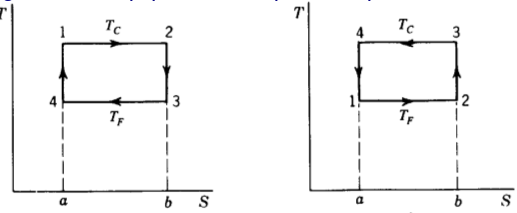
\includegraphics[scale=0.45]{ch7/image1.png}
	\captionof{figure}{Cycles de Carnot (normal et frigo)}
	\end{center}
		Inverser le sens de parcours donne le cycle de Carnot frigorifique.
		
		\subsection{Le chauffage isobare}
		\begin{wrapfigure}[10]{l}{4cm}
		\vspace{-5mm}
		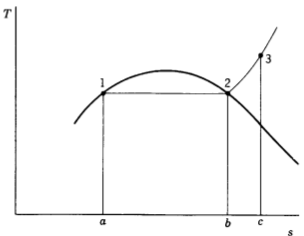
\includegraphics[scale=0.35]{ch7/image2.png}
		\captionof{figure}{ }
		\end{wrapfigure}
		Chauffons de façon isobare réversible une masse de fluide  :
		\begin{equation}
		s_2-s_1 = s_g-s_l = \dfrac{1}{m}\int_1^2 \dfrac{\delta Q}{T} = \dfrac{1}{m}
		\int_1^2 \delta Q = \dfrac{_1q_2}{T} = \dfrac{h_g-h_l}{T}
		\end{equation}
		car pour une isobare en système fermé $\Delta q = \Delta h$. Cette chaleur 
		correspond à l'aire $1-2-b-a-1$. Si on chauffe jusqu'à l'état de vapeur ($2-3$) :
		\begin{equation}
		_2q_3 = \int_2^3 Tds
		\end{equation}
		ce qui est assez délicat à intégrer.
	
		\newpage
		
	\section{Deux relations thermodynamiques importantes}
	Soit une transfo réversible d'un système fermé, par le premier principe 
	\begin{equation}
	dU = \delta Q + \delta WW
	\end{equation}
	La transfo étant réversible (quasi-statique)
	\begin{equation}
	\delta W = -pdV,\qquad \delta Q = TdS
	\end{equation}
	On en déduit
	\begin{equation}
	dU = TdS - pdV
	\end{equation}
	En prenant l'hentalpie $H \equiv U + pV$ et en différenciant 
	\begin{equation}
	dH = dU + pdV + Vdp = TdS + Vdp
	\end{equation}
	On en déduit les formes massiques, hautement utilisées dans ce cours
	\begin{equation}
	\begin{array}{ll}
	du &= Tds- pdv\\
	dh &= Tds + pdv
	\end{array}
	\end{equation}
	
	\section{Transformations ouvertes irréversibles de systèmes fermés}
	Reconsidérons nos deux transformations, sauf que cette fois-ci $A-C$ est 
	irréversible. Pour le cycle réversible :
	\begin{equation}
	\int \dfrac{\delta Q}{T} = \int_1^2 \left(\dfrac{\delta Q}{T}\right)_A + 
	\int_2^1 \left(\dfrac{\delta Q}{T}\right)_B = 0
	\end{equation}
	Pour le cycle de Clausius, l'inégalité s'écrit
	\begin{equation}
		\oint \dfrac{\delta Q}{T} = \int_1^2 \left(\dfrac{\delta Q}{T}\right)_A + 
	\int_2^1 \left(\dfrac{\delta Q}{T}\right)_C < 0
	\end{equation}
	On en déduit
	\begin{equation}
	\int_1^2\left(\dfrac{\delta Q}{T}\right)_C < \int \left(\dfrac{\delta Q}{T}
	\right)_A = \int_1^2 dS = S_2-S_1
	\end{equation}
	On peut écrire
	\begin{equation}
	\dfrac{\delta Q}{T} \leq dS,\qquad\qquad \int_1^2 \dfrac{\delta Q}{T} \leq 
	S_2-S_1
	\end{equation}
	Ces deux relations sont toujours applicable. Si $\delta Q <0$, l'entropie 
	diminuent bien, mais les irréversibilité font toujours grandir celle-ci. 
	"À quantité de chaleur échangée constante, la variation d’entropie est 
	toujours plus élevée pour une transformation irréversible que pour une 
	transformation réversible".
	
	\section{Le travail non compensé}
	Il s'agit du travail perdu à cause des irréversibilités. Considérons un 
	système constitué de deux parties, une vide et une remplie de gaz. 
			\begin{center}
	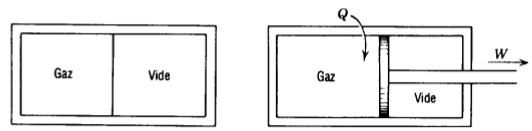
\includegraphics[scale=0.45]{ch7/image3.png}
	\captionof{figure}{ }
	\end{center}	
	Perçons 
	la paroi : aucun travail n'est effectué (température maintenue constante). 
	Comparons avec la situation réversible ou on a 
	\begin{equation}
	\delta Q = TdS,\qquad \delta W^* = pdV
	\end{equation}
	Le travail fourni dans le cas irréversible est plus petit que dans le cas 
	réversible : on a "perdu" du travail 
	\begin{equation}
	(\delta W^*)_{irr} = pdV - \delta W_i^*
	\end{equation}
	Avec le premier principe et le relation de Gibbs
	\begin{equation}
	(\delta Q)_{irr} = (\delta W^*)_{irr} + dU = TdS - \delta W_i^*
	\end{equation}
	on voit que la chaleur reçue est plus petite que dans le cas réversible : 
	c'est la \textit{chaleur non compensée}. En résolvant pour $dS$ :
	\begin{equation}
	dS = \dfrac{\delta Q}{T}+\dfrac{\delta W_i^*}{T}
	\end{equation}
	En comparant avec $dS \leq \dfrac{\delta Q}{T}$, on voit un terme de 
	\textit{production d'entropie}
	\begin{equation}
	dS_i = \dfrac{\delta W_i^*}{T}
	\end{equation}
	
	
	\section{Le principe de l’accroissement de l’entropie}
	Soit une transfo infinitésimale dans un système fermé durant laquelle le 
	système reçoit $\delta Q$ et fourni $\delta W^*$. Le système est à $T$ et 
	le milieu extérieur $T_0>T$. On a 
	\begin{equation}
	dU_{syst} \geq \dfrac{\delta Q}{T}
	\end{equation}
	et pour le milieu extérieur 
	\begin{equation}
	dS_{ext} = -\dfrac{\delta Q}{T_0}
	\end{equation}
	En sommant
	\begin{equation}
	dS_{tot} = dS_{syst} + dS_{ext} \geq \dfrac{\delta Q}{T}-\dfrac{\delta Q}{
	T_0} = \dfrac{\delta Q}{T}\left(1-\dfrac{T}{T_0}\right) > 0
	\end{equation}
	Si $T < T_0$ l'échange est dans l'autre sens ($\delta Q <0$) et on trouve 
	aussi $dS_{tot} \geq 0$, montrant que la variation totale est toujours 
	positive : c'est le \textit{principe d'accroissement d'entropie}. Seule les 
	transfo qui augmente (ou laisse constante) l'entropie globale sont possibles.\\
	
	On peut décomposer cet accroissement global entre contributions interne et 
	externe :
	\begin{equation}
	dS_{syst} =  \dfrac{\delta Q}{T} + dS_i
	\end{equation}
	où $dS_i$ est la production d'entropie due aux irréversibilités internes.
	On a donc
	\begin{equation}
	dS_{tot} = dS_i + \underbrace{\dfrac{\delta Q}{T}\left(1-\dfrac{T}{T_0}\right)
	}_{dS_e} = dS_i+dS_e
	\end{equation}
	où $dS_e$ est la production d’entropie externe due à l'irréversibilité des 
	échanges de chaleur avec le milieu extérieur.
	
	\section{L'entropie d’un solide ou d’un liquide}
	Précédemment, en \textit{Thermodynamique Appliquée} : $dh\approx du \approx cdT$. 
	Comme $du = Tds-pdV$ (et $dh = Tds+vdp$), on a 
	\begin{equation}
	ds \approx \dfrac{du}{T} \approx c \dfrac{dT}{T}
	\end{equation}
	d'où $s_2-s_1 \approx c\ln\left(\dfrac{T_2}{T_1}\right)$.
	
	\section{L’entropie d’un gaz parfait}
	Par Gibbs, $du$, $dh$ et la loi des gaz parfaits : $Tds = du+pdv = c_vdT+pdv$. 
	Après division par $T$ :
	\begin{equation}
	ds = c_v \dfrac{dT}{T}+\dfrac{p}{T}dv = c_v\dfrac{dT}{T} +R\dfrac{dv}{v}
	\end{equation}
	En intégrant, on trouve l'entropie d'un gaz parfait
	\begin{equation}
	s_2 - s_1 = \int_1^2 c_v\dfrac{dT}{T}+R\ln\dfrac{v_2}{v_1}
	\end{equation}
	On aurait aussi pu partir de\footnote{On ajoute $vdp$ dans $dh$ et on le 
	soustrait.} $ds = c_p\dfrac{dT}{T}-\dfrac{v}{T}dp = c_p
	\dfrac{dT}{T}-R\dfrac{dp}{p}$, qui donne une autre relation en intégrant :
	\begin{equation}
	s_2 - s_1 = \int_1^2 c_p\dfrac{dT}{T}-R\ln\dfrac{p_2}{p_1}
	\end{equation}
	Les slides 177-179 montrent comment obtenir le \textit{loi de Laplace}
	\begin{equation}
	pv^k = \text{cste}
	\end{equation}
	
	\section{La transformation polytropique réversible d’un gaz parfait}
	Une transformation $pV^n = \text{cste}$ est dite \textbf{polytropique}. Par 
	exemple, entre deux états 
	\begin{equation}
	p_2V_2^n = p_1V_1^n
	\end{equation}
	Comme le gaz est parfait : $p_1V_1/T_1=p_2V_2/T_2$. En éliminant $V$ ou $P$ 
	on peut obtenir une expression sympa :
	\begin{equation}
	\dfrac{T_2}{T_1}=\left(\dfrac{p_2}{p_1}\right)^{\frac{n-1}{n}} = \left(\dfrac{
	V_1}{V_2}\right)^{n-1}
	\end{equation}
	Des applications sont données slide 181.
	
	
	\section{Le second principe de la thermodynamique pour les systèmes ouverts}
	On faisant comme en 5.10, on peut obtenir la douce relation suivante 
	\begin{equation}
	\dfrac{dS_F}{dt} = \dfrac{dS_O}{dt} + \oint_S\rho s(\vec{c}-\vec{b_O}).\vec{n}\ 
	dS = \dfrac{dS_O}{dt} + \sum \dot{m_s}s_s - \sum \dot{m_e}s_e
	\end{equation}
	On avait vu que le second principe appliqué aux systèmes fermés s'écrit 
	\begin{equation}
	dS = \dfrac{\delta Q}{T}+dS_i
	\end{equation}
	mais c'était dans le cas ou l'on avait des variables uniformes, ce qui n'est 
	pas souvent le cas pour $T$ sur les frontières ou un échange de chaleur se produit. 
	Il faut remplacer $\delta Q/T$ par une somme sur chaque élément de frontière dont 
	la température est différente. A la limite infinitésimale, on obtiendrait : 
	\begin{equation}
	\dfrac{\delta Q}{T} \leftarrow \oint_{\mathcal{A}} \dfrac{d\Phi}{T}d\mathcal{A}
	\end{equation}
	En rassemblant tout, on obtient alors
	\begin{equation}
	\dfrac{dS_O}{dt} +\sum\dot{m_s}s_s - \sum \dot{m_e}s_e = \sum \dfrac{\dot{Q}}{T}
	+\dot{S_i} = \oint_{\mathcal{A}}\dfrac{\Phi}{T}d\mathcal{A}+\dot{S_i}
	\end{equation}
	
	\section{Les systèmes ouverts en régime permanent et les systèmes ouverts avec
			 écoulement uniforme}
	Si le système est permanent, l'expression se simplifie en : 
	\begin{equation}
	\sum \dot{m_s}s_s - \sum \dot{m_e}s_e = \sum\dfrac{\dot{Q}}{T}+\dot{S_i}
	\end{equation}
	Pour une transfo adiabatique :
	\begin{equation}
	s_s-s_e = \dfrac{\dot{S_i}}{m}\geq 0.
	\end{equation}
	Pour le système ouvert avec écoulement uniforme :
	\begin{equation}
	\dfrac{d(ms)_O}{dt} + \sum \dot{m_s}s_s - \sum \dot{m_e}s_e = \dfrac{\dot{Q}}{T} 
	+\dot{S_i}
	\end{equation}
	
	
	\section{Les transformations réversibles des systèmes ouverts en régime permanent}
	Cherchons une expression du travail échangé par un système ouvert permanent dans le 
	cas d'une transformation réversible. On avait trouvé, dans le cas d'une entrée/sortie :
	\begin{equation}
	\left(h+\dfrac{c^2}{2}+gz\right)_s - \left(h+\dfrac{c^2}{2}+gz\right)_e = q+w
	\end{equation}
	et le second principe
 	\begin{equation}
 	\dot{m}(s_s-s_e)=\sum\dfrac{\dot{Q}}{T}+\dot{S_i}\geq \sum\dfrac{\dot{Q}}{T}
 	\end{equation}
 	Voyons maintenant deux transformations réversibles:
 	\begin{enumerate}
 	\item \textit{Transformation adiabatique}.\\
 	Le second principe se réduit à $s_s=s_e$. Avec la relation de Gibbs $dh = Tds+vdp, 
 	h_s-h_e = \int_e^s vdp$ et on a 
 	\begin{equation}
 	w = \int_e^s vdp +\dfrac{c_s^2+c_e^2}{2} + g(z_s-z_e)
 	\end{equation}
 	\item \textit{Transformation isotherme}.\\ 	
 	La température est uniforme : $\sum \dfrac{\dot{Q}}{T} = \dfrac{\dot{Q}}{T}=\dot{m}
 	\dfrac{q}{T}$ et le second principe devient $s_s-s_e = \dfrac{q}{T}$. Par application 
 	de la même relation de Gibbs
 	\begin{equation}
 	h_s-h_e = T(s_s-s_e) + \int_e^s vdp
 	\end{equation}
 	l'expression du travail $w$ est identique.
 	\end{enumerate}
 	Notre expression $w$ est donc bonne pour toute transfo réversible de systèmes ouvert 
 	en régime permanent. Cette expression est employée pour tous les systèmes ouverts avec
	échange de travail comme les turbomachines. Si les variations d’énergie cinétique et 
	potentielle sont négligeables :
	\begin{equation}
	w = \int_e^s vdp
	\end{equation}
	Le travail en système ouvert est directement lié à la variation de pression. On en 
	déduit que s'il n'y a pas de travail, la pression reste constante. Petit exemple slide 
	191.
	
	\section{Principe d’accroissement de l’entropie pour un système ouvert}
	Suivons un raisonnement semblable à celui fait précédemment mais pour un système 
	ouvert dont la variation d'entropie s'écrit
	\begin{equation}
	\dfrac{dS_{syst}}{dt}+\sum \dot{m_s}s_s - \sum \dot{m_e}s_e = \sum\dfrac{\dot{Q}}{T}+\dot{S_i}
	\end{equation}
	Le milieu extérieur est aussi un milieu ouvert 
	\begin{equation}
	\dfrac{dS_{ext}}{dt}-\sum \dot{m_s}s_s + \sum \dot{m_e}s_e = -\sum\dfrac{\dot{Q}}{T_0}
	\end{equation}
	En sommant les deux équations :
	\begin{equation}
	\dfrac{dS_{tot}}{dt} = \dfrac{dS_{syst}}{dt}+\dfrac{dS_{ext}}{dt} = \underbrace{
	\sum\dfrac{\dot{Q}}{T}-\dfrac{\sum \dot{Q}}{T_0}}_{\dot{S_e}} + \dot{S_i} = \dot{S_e}
	+\dot{S_i} > 0
	\end{equation}
	avec $\dot{S_e}$ toujours positif : c'est le taux de production d'entropie externe due 
	à l'irréversibilité de l'échange de chaleur.\\
	Pour un système ouvert en régime permanent, l’entropie du système est constante\footnote{??} :
	\begin{equation}
	\dfrac{dS_{tot}}{dt} = \dfrac{dS_{ext}}{dt} = \sum\dot{m_s}s_s-\sum\dot{m_e}s_e - 
	\dfrac{\dot{Q}}{T_0}
	\end{equation}
	Si l'écoulement est uniforme, on intégrera cette relation.
	
	\section{Les rendements}
	Cette partie n'est pas détaillée ici, tout est clair et limpide avec le formulaire ! Et 
	j'avoue avoir un peu la flemme de \LaTeX iser tous ça pour pas grand chose!
	
	
	